\chapter{前景约束的欧拉影像动作放大技术}
\label{chap:fc-evm}

针对第 \ref{chap:previous} 章中所介绍的几种动作放大方法的不足,本文提出一种前景约
束的欧拉影像动作放大方法,该方法在欧拉视角的动作放大方法的基础上,结合了拉格朗日
视角的特点,通过使用目标跟踪技术,将放大区域限制在由用户选定的感兴趣区域上,再通
过使用前景分割技术,将动作结果与原图像的,将放大区域进一步限制在
感兴趣区域中的前景区域。数学上,本文使用四元数矩阵一次性处理视频的彩色序列帧的三
个通道,具备更好的完整性。

本文的算法包括如下几个步骤:

\begin{compactenum}
\item 选择感兴趣区域(Region of Interest,ROI)。用户在参照帧中手动框选一个感兴
  趣的区域(如人脸),作为后续的跟踪目标和前景分割的初始区域;
\item 区域跟踪和前景提取。使用目标跟踪算法对感兴趣区域进行跟踪,并从跟踪区域中提取出前景掩码;
\item 局部欧拉影像动作放大。对跟踪区域进行局部的欧拉影像动作放大;
\item 金字塔率混合。将放大结果与原图进行金字塔混合;
\item 合成视频。合成最终视频。
\end{compactenum}

本文的算法框架如图 \ref{fig:fc-evm-frameworks} 所示。出于论述上的简单,本文主要采
用线性的欧拉影像动作放大算法进行动作放大。该算法也可以替换成基于相位的方法,以得
到最优的放大结果。

\begin{landscape}
  ~\\
  ~\\
  \begin{figure}[htbp]
  \centering
  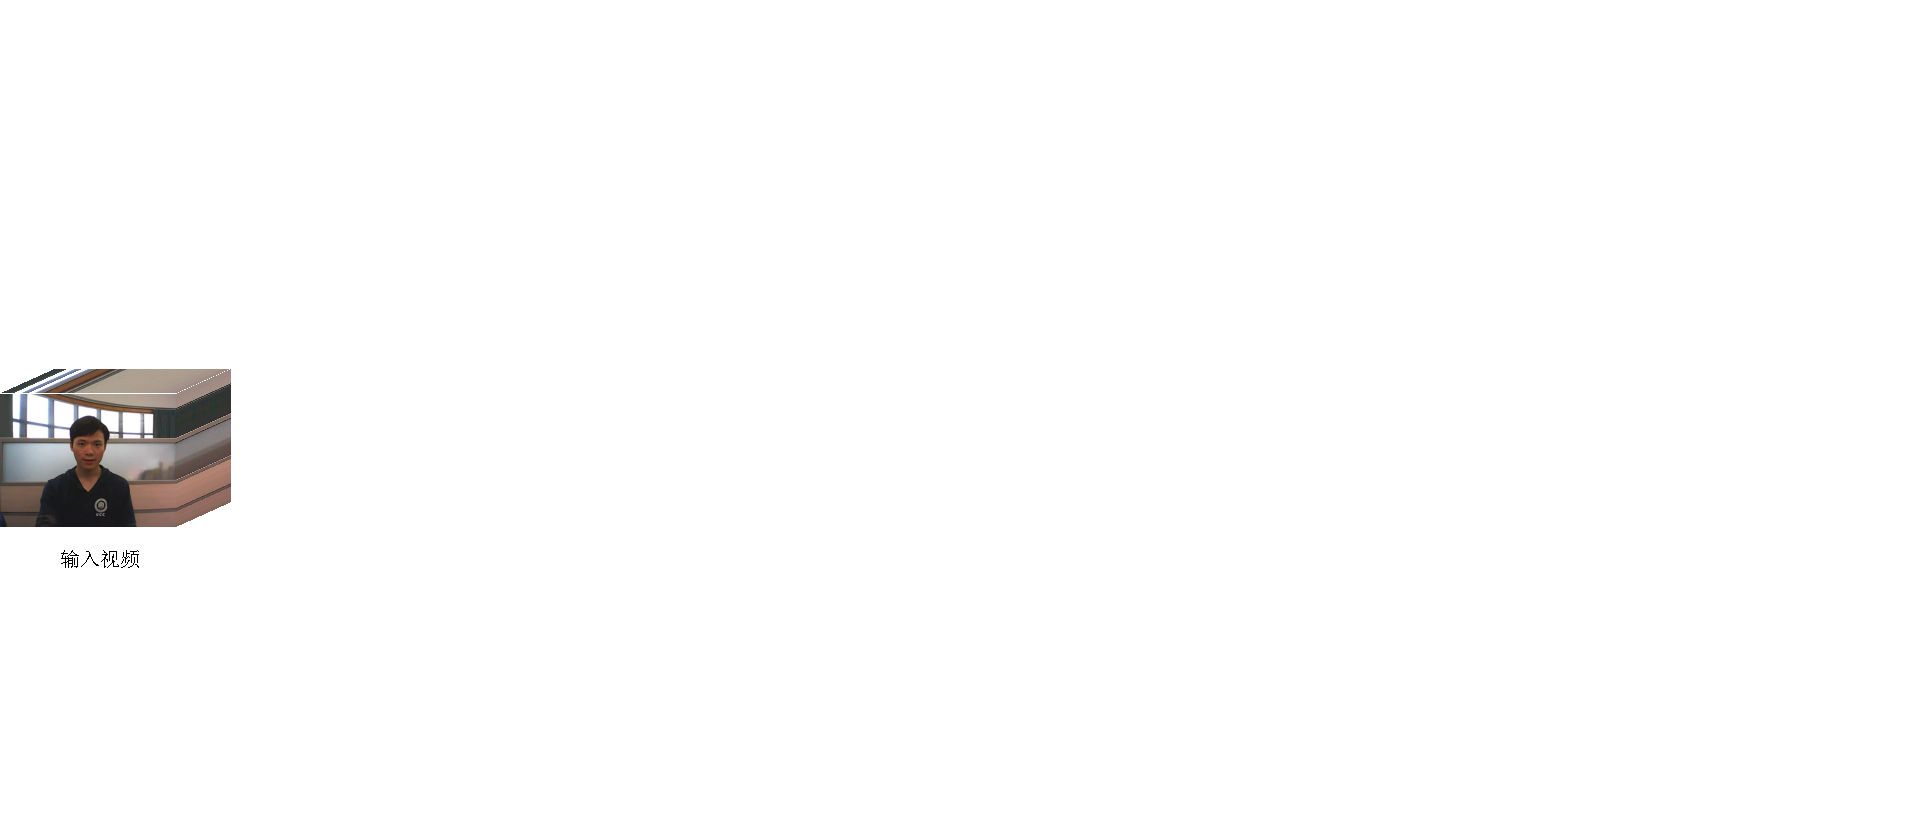
\includegraphics[width=1.5\textwidth]{fc-evm.pdf}
  \caption{前景约束的欧拉动作放大算法框架图}
  \label{fig:fc-evm-frameworks}
\end{figure}
\end{landscape}

\section{选择感兴趣区域}
\label{sec:choose-roi}



\section{局部欧拉影像动作放大}
\label{sec:local-evm}



%%% Local Variables: 
%%% mode: latex
%%% TeX-master: "../thesis"
%%% End: 
